\chapter{System design and validation} \label{ch10}
With the concept and requirement for the system established in section \ref{sec:synth} and necessary theoretical knowledge obtained through chapter \ref{ch4} to \ref{ch7} system design are to be set up in this chapter. Test for validation of each unit will be carried out and documented along with the design process according to the test specifications in section \ref{sec:testspec}. One section is allocated to each software unit in the application cp. section \ref{sec:testspec}.The chapter concludes with a test of the final system followed by an evaluation.  \\


\section{Fourier transformation - FFT}
\section{FFT}
This section describes the implementation of the FFT discussed in section \ref{sec:FFT}, which uses an implementation of the DFT discussed in section \ref{sec:DFT}. The implementation of the FFT is assessed by comparing both the computational efforts and the results of the implementations of the DFT and FFT compared to Numpy's FFT. The results are expected to be similar since the FFT is a fast way of calculating the DFT.

\subsection{Implementation of the FFT}
Firstly, the implementation of the DFT is described in the following algorithm.
\begin{algorithm}
\caption{DFT algorithm}
\label{DFTalg}
\begin{algorithmic}[1]
\State $N =$length of $x$ \Comment{Number of samples to be computed}
\Procedure{Compute DFT}{x,N}
	\State{$X = $np.zeros$(N,$dtype=complex$)$}
	\For{k between 0 and length of signal}
		\State{$a = 0 + 0\cdot j$} \Comment{$a$ is zero but of type complex}
		\For{n between 0 and N}
			\State{$a += x[n]\cdot \exp(-2\cdot \pi\cdot j 					\cdot k \cdot n/$float$(c))$}
			\State{$X[k] = a$}
		\EndFor
	\EndFor
	\State {Return $X$}
\EndProcedure
\end{algorithmic}
\end{algorithm}

The implementation of the FFT shown in the following algorithm uses a function to make sure that the number of samples to be computed is a power of 2 (as described in section \ref{sec:FFT}). This function asks if $N$ is positive and a power of 2. If not, the function returns a False-statement, which raises a \textit{Valueerror} in the FFT algorithm. However, the FFT function from the Numpy-package uses zeropadding to modify a signal of arbitrary length into a signal with a length that is a power of 2. That has not been implemented in the FFT shown below. In the FFT algorithm shown below, the signal is divided into even and odd samples if the signal is more than 2 samples long, which are computed separately by using the FFT itself; if the number of even (and odd) samples are still more than 2 the samples are divided even further until the number of even (and odd) samples are 2. These samples are then computed by the DFT described in algorithm \ref{DFTalg}. After dividing the samples into even and odd samples the twiddle factor is multiplied appropiately (as described in section \ref{sec:FFT}), and eventually the Numpy-function \textit{concatenate} is used to join the arrays back together.\martin{Hvad betyder \& i algoritmen?}
\begin{algorithm}
\caption{FFT algorithm}
\label{FFTalg}
\begin{algorithmic}[1]

\Procedure{Power of 2}{N}
	\State{Return $N$!=$0$ and $(N \& (N - 1)) == 0$}
\EndProcedure

\Procedure{Compute FFT}{x}
	\State $N$ = length of $x$ 
	\If{Power of 2($N$) == False }
		\State{Raise Valueerror(``N should be a power of 2.'')}
	\ElsIf{$N$ == 2}
		\State{Return DFT($x$,$N$)} \Comment{$x$ is the signal}
	\Else
		\State{$X_{e} = FFT(x[::2])$} \Comment{The even 				samples}
		\State{$X_{o} = FFT(x[1::2])$} \Comment{The odd 				samples}
		\State{$factor = \exp(-2j\cdot \pi \cdot 						$np.arange$(N) / N)$} \Comment{The twiddle 			factor}
		\State{Return np.concatenate$([X_{e} + factor[: 	N/ 2] \cdot X_{o}, X_{e} +  factor[N / 2:] \cdot X_{o}])$}
	\EndIf
\EndProcedure
\end{algorithmic}
\end{algorithm}

\subsection{Test of the FFT}
The FFT algorithm above is compared to both the DFT algorithm and the FFT function from the Numpy-package by measuring how long it takes for the functions to compute different amounts of random numbers. This is shown in table \ref{tab:FTcompare}. Furthermore, the algorithms are compared by their outputs.

\begin{table}[H]
\centering
\begin{tabular}{|l|l|l|l|}
\hline
Type / $N$ & DFT	   & FFT 	 & Numpy's FFT \\ \hline
$2^9$  	   & $1.03$    & $0.01$  & $\sim 0.00$ \\ \hline
$2^{10}$   & $4.43$    & $0.02$  & $\sim 0.00$ \\ \hline
$2^{11}$   & $17.36$   & $0.03$  & $\sim 0.00$ \\ \hline
$2^{12}$   & $69.42$   & $0.07$  & $\sim 0.00$ \\ \hline
$2^{13}$   & $290.89$  & $0.18$  & $\sim 0.00$ \\ \hline
$2^{14}$   & $1206.85$ & $0.27$  & $\sim 0.00$ \\ \hline
\end{tabular}
\caption{Times in seconds it take for the implementations of the DFT, the FFT and Numpy's FFT to compute $N$ random numbers. Processor used: Intel Core I5 generation 5 with CPU of 2.20 GHz.}
\label{tab:FTcompare}
\end{table}

Table \ref{tab:FTcompare} shows that the time the DFT takes to compute the $N$ numbers grows rapidly, whereas either of the FFTs take less than a second. The values for Numpy's FFT are rounded off to zero, and this function's ability to rapidly perform the computations is due to the fact that Numpy actually performs the computations in C, where the code is already compiled and runs directly on the CPU. On the other hand, Python is an interpreted language, which means that each line of the code has to be translated before it can be run. However, that obviously does not mean that the implementation of the FFT shown above is slow, and it is certainly much faster than the implementation of the DFT. \\
It is furthermore interesting to examine whether this result corresponds to the theoretical relation of the computational complexities. From section \ref{sec:FFT} the theoretical numbers of arithmetic operations required to compute the DFT and FFT are $N^2$ and $N\log_2(N)$, respectively. The relation $\frac{N^2}{N \cdot \log_2(N)}$ of these computational complexities equals $\frac{N}{\nu}$ for $N = 2^\nu, \nu \in \mathbb{N}$, which is a 


  
For $N=2^9$ this gives an approximate relation of the FFT being $57$ times faster than the DFT but the actual relation is $103/1$ from table \ref{tab:FTcompare}. From this the computation of the implemented FFT is approximately twice as fast as found theoretically compared to the implemented DFT, which is due to the number of computations and the computer's processing time cannot be directly compared \martin{Martin udvider sammenligningen af tallene}. \\
\\
The implementation of the FFT and Numpy's FFT should also be compared for larger number of samples $N$ since e.g. $N = 2^{19}$ is 11.89 seconds with a sampling frequency of 44100 Hz, which is a reasonable length of an audio file from the recordings described in appendix \ref{recordings}. The DFT will obviously take too long and is therefore not included in the comparison in table \ref{tab:FT2compare}.

\begin{table}[H]
\centering
\begin{tabular}{|l|l|l|l|}
\hline
Type / $N$ & FFT	   & Numpy's FFT \\ \hline
$2^{18}$   & $5.15$    & $0.03$ \\ \hline
$2^{19}$   & $9.79$    & $0.04$ \\ \hline
$2^{20}$   & $19.74$   & $0.14$ \\ \hline
$2^{21}$   & $40.31$   & $0.26$ \\ \hline
$2^{22}$   & $79.59$   & $0.56$ \\ \hline
$2^{23}$   & $159.39$  & $1.08$ \\ \hline
\end{tabular}
\caption{Times in seconds it take for the implementation of the FFT and Numpy's FFT to compute $N$ random numbers. Processor used: Intel Core I5 generation 5 with CPU of 2.20 GHz.}
\label{tab:FT2compare}
\end{table}

Obviously, the implementation of the FFT takes rather long for large numbers of samples, whereas Numpy's FFT only takes a little more than a second. It should be noted that the results above cannot be reproduced exactly since the numbers are random and the same amount of different numbers results in slightly different times of computations. Also, one might check the validity of the DFT and FFT algorithms by comparing the result of the algorithms and Numpy's FFT by using the Numpy function \textit{np.allclose}. An example is \textit{np.allclose(FFT(x),np.fft.fft(x))}, which returns a True-statement if the results of $FFT(x)$ described in algorithm \ref{FFTalg} and Numpy's FFT are similar to a certain degree$^[$\footnote{See also the documentation for the \textit{allclose}-function on \href{https://docs.scipy.org/doc/numpy/reference/generated/numpy.allclose.html}{https://docs.scipy.org}.}$^]$. This was always the case in the comparison of the implementations of the DFT, the FFT and Numpy's FFT described above.
\\ \\
Therefore, the implementation of the DFT and FFT described in algorithm \ref{DFTalg} and \ref{FFTalg}, respectively, returns the exact same values as Numpy's FFT. The DFT is obviously extremely slow for even rather small numbers of samples, and the FFT is also rather slow compared to Numpy's FFT for large numbers of samples.
\\ \\
Because Numpy's FFT is so much faster than the implemented FFT and because Numpy's FFT is capable of zeropadding and thus computing a signal of any length, it is decided to use Numpy's FFT in the future processings of the signals in this report \martin{Nyt. \textregistered}.

\section{Filter}
The filter design process is documented in this section, which includes determination of filter specifications, implementation and test. As stated in section \ref{sec:filtervalg} a bandpass FIR filter of type I designed with use of a Kaiser window is wanted.

\subsection{Specifications of filter} \label{sec:FIRspec} 
The purpose of this filter is to remove all frequencies outside the passband of the filter.  \\
Due to the frequency analysis in section ~\ref{sec:single} the main energy in the analysed signals is located within a frequencyband from 75 Hz to 1000 Hz.  
By letting the cut-off frequencies $f_c$ of the filter be respectively 75 Hz and 1000 Hz, this makes the passband of the filter. \\ 
According to section \ref{subsec:FIR} the Kaiser window can be determined from specifications of the allowed transition width $tw$ and peak approximation error $\delta$ of the amplitude in the pass- and stopbands. \\ 
By the frequency analysis of different types of noise it is found that the frequency spectrum of the music signal leis within the frequency spectrum of the noise which verifies the need of a narrow transitionband. However, the narrower transitionband means the higher order of filter is needed, which gives more computations, and hence it is not realistic to let the width of the transitionband go toward zero.  \\
The maximum allowed width of the transitionband $tw$ and peak approximation error in amplitude $\delta$ is determined as
\begin{align}
tw = 20 \ Hz, \ \ \ \ \  \delta = 0.05. 
\end{align}
The amplitude response of the ideal filter is sketched in figure \ref{fig:spec_Hd} along with the boundaries for the real filter as provided by the defined specifications.      

\begin{figure}[H]
\centering
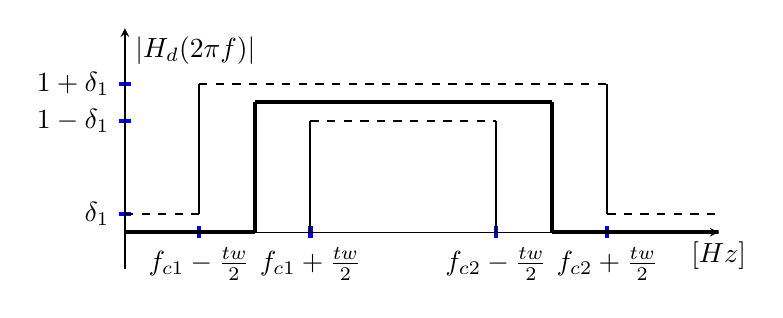
\begin{tikzpicture}[scale=1]
\begin{axis}[every tick/.style={blue, ultra thick}, 
scale=1.1,
unit vector ratio*=1 1 1,
axis lines = middle,
x label style={at={(current axis.right of origin)},anchor=north},
xlabel={$[Hz]$},
xtick={2,5,10,13},
xticklabels={$f_{c1}-\frac{tw}{2}$,$f_{c1}+\frac{tw}{2}$,$f_{c2}-\frac{tw}{2}$,$f_{c2}+\frac{tw}{2}$},
ytick={0.5,3,4},
yticklabels={$\delta_1$,$1-\delta_1$,$1+\delta_1$},
xmin=0,
xmax=16,
ymin=-1,
ymax=5.5]
\node at (axis cs:1.9,4.9) {$|H_d(2\pi f)|$};
\draw[line width=0.5mm](axis cs:0,0)--(axis cs:3.5,0);
\draw[line width=0.5mm](axis cs:3.5,0)--(axis cs:3.5,3.5);
\draw[line width=0.5mm](axis cs:3.5,3.5)--(axis cs:11.5,3.5);
\draw[line width=0.5mm](axis cs:11.5,3.5)--(axis cs:11.5,0);
\draw[line width=0.5mm](axis cs:11.5,0)--(axis cs:16,0);
\draw[line width=0.25mm, dashed](axis cs:0,0.5)--(axis cs:2,0.5);
\draw[line width=0.25mm, dashed](axis cs:13,0.5)--(axis cs:16,0.5);
\draw[line width=0.25mm, dashed](axis cs:5,3)--(axis cs:10,3);
\draw[line width=0.25mm, dashed](axis cs:2,4)--(axis cs:13,4);
\draw[line width=0.25mm](axis cs:2,0.5)--(axis cs:2,4);
\draw[line width=0.25mm](axis cs:5,0)--(axis cs:5,3);
\draw[line width=0.25mm](axis cs:10,0)--(axis cs:10,3);
\draw[line width=0.25mm](axis cs:13,4)--(axis cs:13,0.5);
%\draw[line width=0.5mm](axis cs:4,0.5)--(axis cs:7,0.5);
%\node at (axis cs:1,1.5) {Passband};
%\node at (axis cs:3,1.5) {Transition};
%\node at (axis cs:5.0,1.5) {Stopband};
\end{axis}
\end{tikzpicture}
\caption{Amplitude response of ideal filter within the boundaries for the amplitude response of the realizable filter as given by the defined specifications.}
\label{fig:spec_Hd}
\end{figure}

\subsection{Implementation of filter}
The implementation of the filter basically follows algorithm \ref{alg:FIR}. The ideal impulse response is defined as the inverse Fourier transformation of the ideal filter specified in figure \ref{fig:spec_Hd}. The derivation of the ideal impulse response of a bandpass filter is shown in appendix \ref{appC}. From the given specifications the shape parametere of the kaiser window becomes $\beta \approx 1.5$ which gives a filter order of 2766. Figure \ref{fig:FIRimpulse} show the impulse response of the filter. Figure \ref{fig:freq_filt1} illustrates a plot of the amplitude response corresponding to the filter in the frequency domain. Figure \ref{fig:freq_filt2} illustrates a close-up view of the left transitionband, showing the ripples in the stop- and passband. The boundaries from the specifications are marked by the green lines. It is seen that the specifications are fulfilled. 
\begin{figure}[h]
\centering 
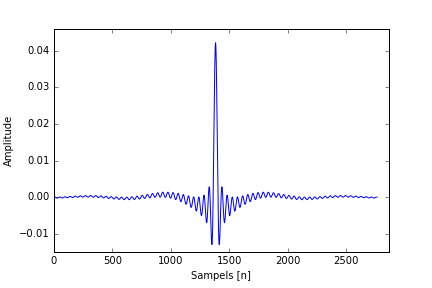
\includegraphics[scale=0.4]{figures/filtertest/impulse.png}
\caption{Impulse response of filter with order $M=2766$}
\label{fig:FIRimpulse}
\end{figure}
       
\begin{figure}[h]
\centering
\begin{subfigure}{0.49\textwidth}
\centering
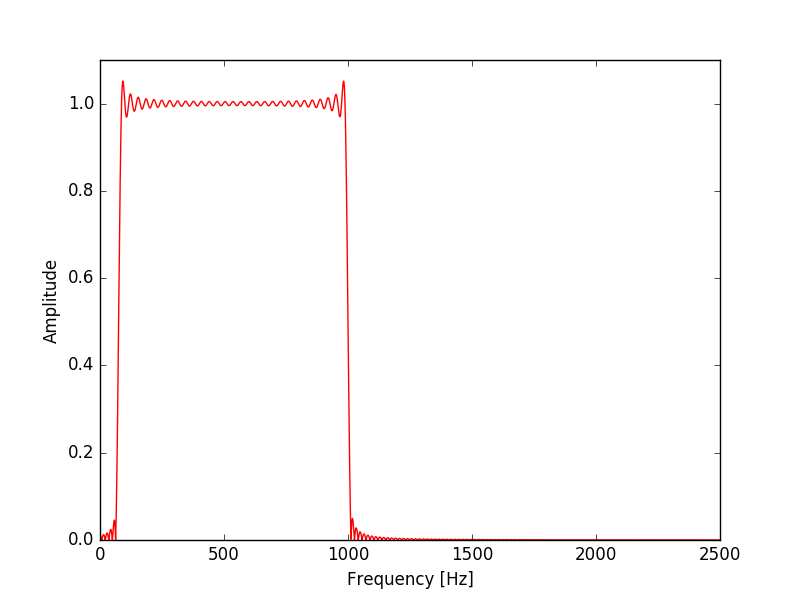
\includegraphics[width=\textwidth]{figures/filtertest/freq_response1.png}
\caption{}
\label{fig:freq_filt1}
\end{subfigure}
\begin{subfigure}{0.49\textwidth}
\centering
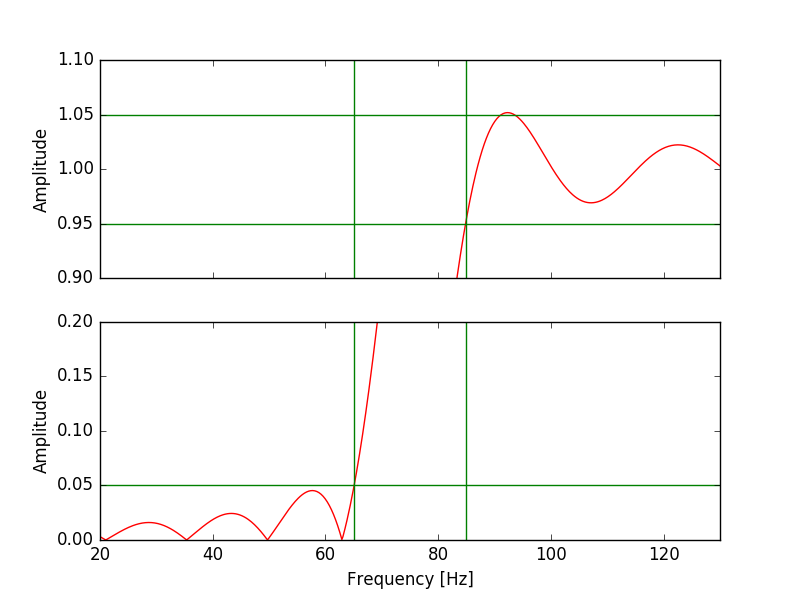
\includegraphics[width=\textwidth]{figures/filtertest/freq_response2.png}
\caption{}
\label{fig:freq_filt2}
\end{subfigure}
\caption{(a) Amplitude response of filter. (b) Close-up view of amplitude response of filter, showing top and bottom of one transitionband.}
\label{fig:freq_filt}
\end{figure}

\begin{algorithm}[H]
\caption{Compute type I FIR filter}
\label{alg:FIR}
\begin{algorithmic}[1] 
\Procedure{Compute kaiser window $w$}{}
\State $A=-20\log_{10}(\delta)$ \Comment{$21 \leq A \leq 50$}
\State $\beta = 0.5824(A-21)^{0.4} + 0.07886(A-21)$ \Comment {Shape parameter}
\State $M = (A-8)/(2.285 \cdot \frac{tw}{f_s} 2\pi)$ \Comment {Filter order, round to upper even int.}
\State $N = M+1$ \Comment {Length of filter}
	\For {each $i$ in length of $N$}
		\For {each $j$ in length of $M$}
			\State $ sum_n + = \ (\frac{1}{j!})^2 \left( \left( \frac{\beta}{2} \sqrt{\left(1 - \left( \frac{2 \cdot i}{N-1}\right) - 1\right)^2}\right)^{2j}\right)$
			\State $ sum_d + = \ (\frac{1}{j!})^2 \left( \frac{\beta}{2}\right)^{2j}$
		\EndFor
		\State $w[i]=\frac{sum_n}{sum_d}$
	\EndFor
	\State Return $w$, $M$
\EndProcedure
\\
\Procedure{Compute ideal impulse response $h_d$}{}
   \For {each $i$ in length of $N$}
        \If {$i == \frac{M}{2}$}
        		\State $h_d[i] = 2( \frac{f_{c2}}{f_s} - \frac{f_{c2}}{f_s})$
        	\Else 
        		\State  $h_d[i] = \frac{1}{ (\pi (i - \frac{M}{2}))}(\sin(\frac{f_{c2}}{f_s} 2 \pi (i - \frac{M}{2})) - (\sin(\frac{f_{c1}}{f_s} 2 \pi (i - \frac{M}{2}))))$ 
          	\EndIf 
  	\EndFor
  	\State Return $h_d$
\EndProcedure
\\
\Procedure{Compute impulse response $h$}{}
	\State Return $h = h_d \cdot w$ \Comment{Windowed impulse response}
\EndProcedure


\end{algorithmic}
\end{algorithm}

\subsection{Test of the filter}
The implemented filter is tested according to the test specifications described in section \ref{sec:testspec}. Figure \ref{fig:SIGNAL} shows the frequency spectrum of the single low E tone with additive noise in form of a beat of hands clapping. Figure \ref{fig:filt_SIGNAL} shows the filtered signal. Note that the frequency spectrum are only showed from 0 to approximately 2200 Hz.  

\begin{figure}[H]
\centering
\begin{subfigure}{0.49\textwidth}
\centering
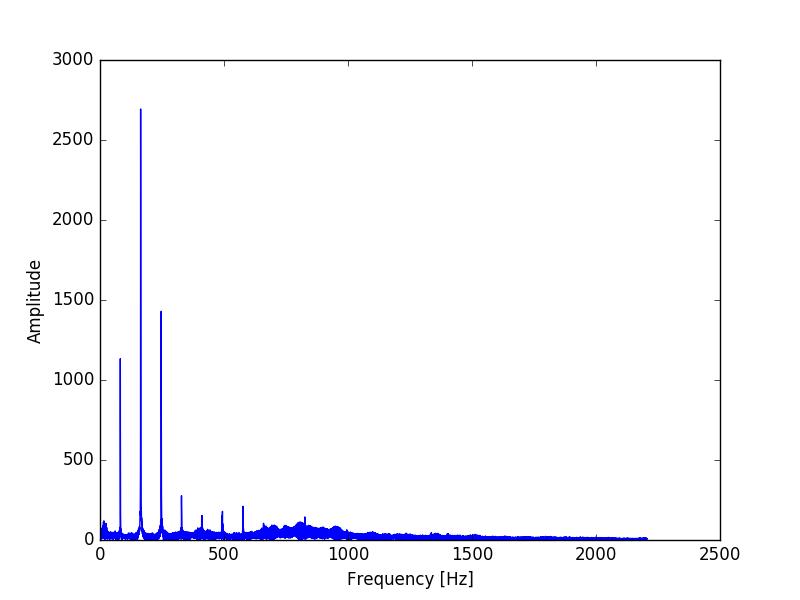
\includegraphics[width=\textwidth]{figures/filtertest/SIGNAL.png}
\caption{}
\label{fig:SIGNAL}
\end{subfigure}
\begin{subfigure}{0.49\textwidth}
\centering
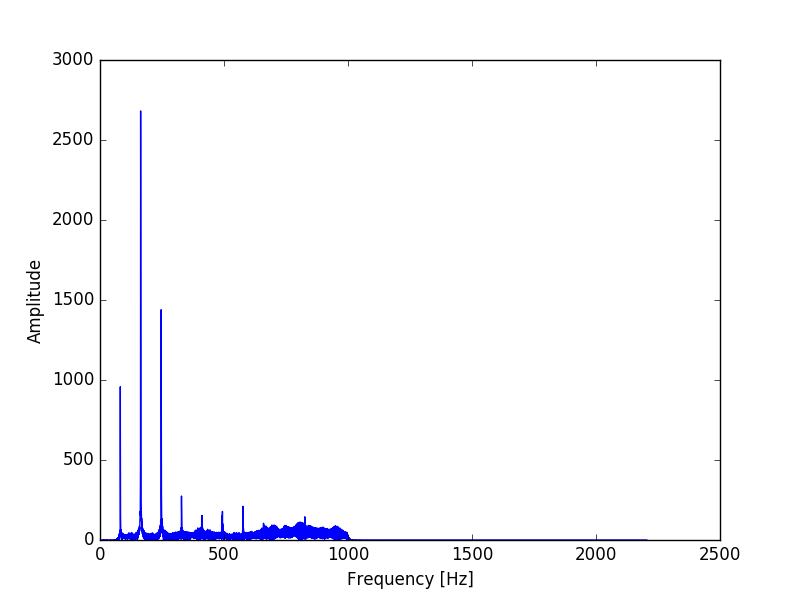
\includegraphics[width=\textwidth]{figures/filtertest/filt_SIGNAL.png}
\caption{}
\label{fig:filt_SIGNAL}
\end{subfigure}
\caption{(a) Frequency spectrum of signal with noise. (b) Frequency spectrum of filtered signal.}
\label{fig:test_res}
\end{figure}
As described in the specifications the filter is designed to remove all frequencies outside the frequencyband from 75 Hz to 1000 Hz. It is seen by comparing figure \ref{fig:SIGNAL} and figure \ref{fig:filt_SIGNAL} that the frequencies outside the passband appears to be zero and that the amplitudes of the remaining frequencies are appropriately the same. \\
By this the designed filter of order 2766 fulfil the specifications and the implementation of the filter works as intended. \\

\section{STFT}

\section{Spectrogram}

\section{Integration validation}

\section{Final system test}

